\documentclass[11pt]{report}
\usepackage{graphicx}
\usepackage[a4paper, portrait, margin=1.6cm]{geometry}
\usepackage{enumitem}
\hyphenpenalty 80
\usepackage{lmodern}
\usepackage[T1]{fontenc}
\usepackage[hidelinks]{hyperref}
\newcommand{\ts}{\textsuperscript}

\begin{document}
\pagenumbering{gobble}
\hspace*{-\parindent}\hspace{-1em}
\begin{tabular}{p{3.8cm} p{13cm}}
    \vspace{0pt} 
    {%
	\setlength{\fboxsep}{0pt}%
	\setlength{\fboxrule}{0.75pt}%
    \fbox{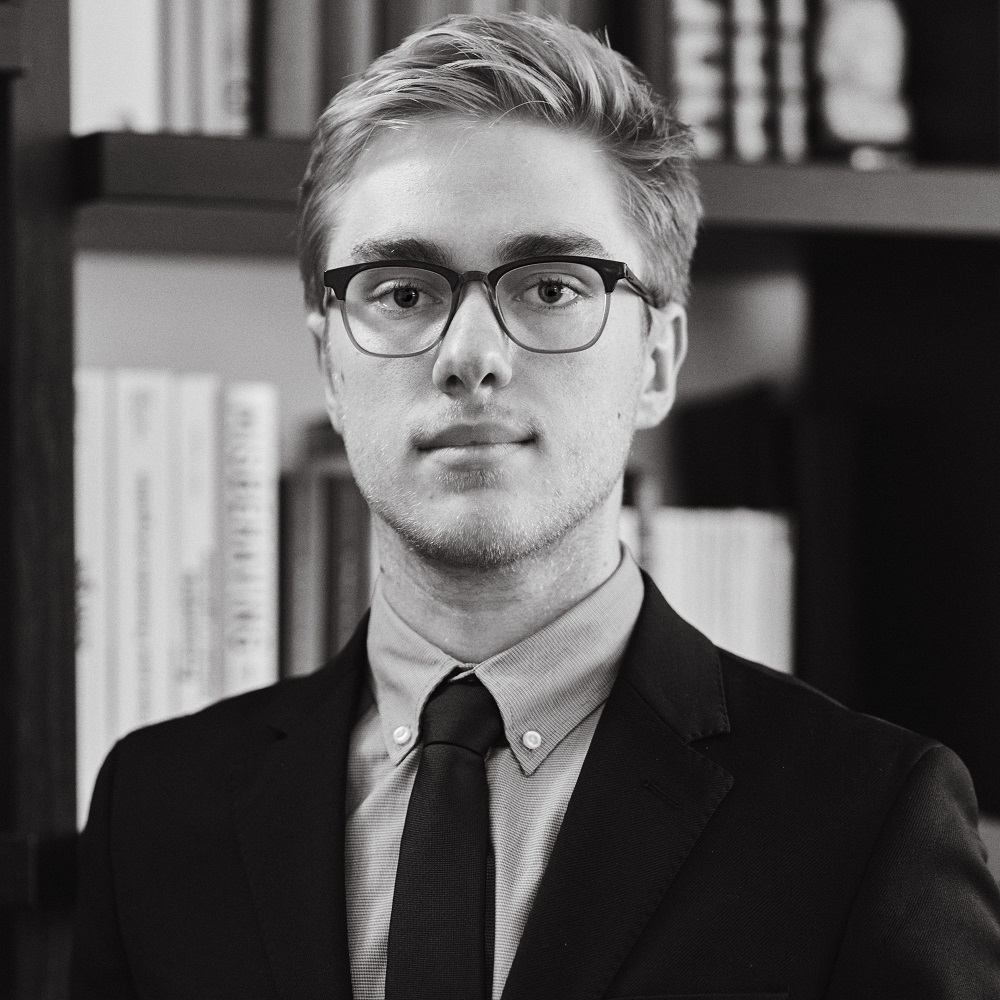
\includegraphics[scale=0.445]{./content/picture.jpg}}%
    }%
    & 
    \vspace{0pt}
	\begin{Large}\textbf{PATRYK WISNIEWSKI}\end{Large}
	\newline \emph{Étudiant ingénieur économiste}
	\newline
	\newline \makebox[2cm][l]{Addresse :}155 Avenue Pierre Brossolette
	\newline \makebox[2cm][l]{}92120 Montrouge, France
	\newline \makebox[2cm][l]{Email :}\href{mailto:patryk@pwisniewski.com}{\underline{patryk@pwisniewski.com}}
	\newline \makebox[2cm][l]{Linkedin :}\href{https://linkedin.com/in/pwisniewski02}{\underline{pwisniewski02}}
	\newline \makebox[1.75cm][l]{Mobile :} +33 6 95 30 31 18
	\end{tabular}

\begin{flushleft}
\raisebox{-.6ex}{FORMATION} \hrulefill
\end{flushleft}

	
\noindent\textbf{Programme ingénieur \textbar\space Économie et Statistiques}
\hfill
\textbf{08/2023 - présent} \\
\emph{ENSAE - Institut Polytechnique de Paris}\\
Programme ingénieur multidisciplinaire combinant un niveau élevé de mathématiques appliquées, statistiques,  économie, économétrie, informatique et machine learning. \\

\noindent\textbf{Master 1 \textbar\space Quantitative Economics}
\hfill
\textbf{08/2022 - 05/2023} \\
\emph{Université Paris Dauphine - PSL}\\
Master entièrement enseigné en anglais avec des cours avancés en microéconomie, macroéconomie, théorie des jeux et économétrie, ainsi que des enseignements supplémentaires en science des données. Projet de M1 sur l'économie de la vie privée et les asymétries d'informations entre individus et plateformes.\\
\\
\noindent\textbf{Licence \textbar\space Magistère d'Économie}
\hfill
\textbf{09/2019 - 06/2022} \\
\emph{Paris 1 Panthéon Sorbonne \& PSE}\\
Licence obtenue dans le magistère d'économie, un programme sélectif principalement axé sur les enseignements quantitatifs comprenant des mathématiques avancées, des statistiques et de l'économétrie. Mémoire sur l'effet de tremplin des contrats à court terme sur le marché du travail français.

	\begin{flushleft}
	\raisebox{-.6ex}{EXPÉRIENCES PROFESSIONNELLES} \hrulefill
	\end{flushleft}


\noindent\textbf{École des Mines de Paris} \hfill Paris, France\\[0.1cm]
\textbf{Assitant de recherche} (temps partiel)\hfill \textbf{09/2023 - présent} \\
Collaboration avec une équipe de chercheurs dans le cadre de la rédaction rapport sur la décarbonisation du secteur manufacturier français. Création de statistiques descriptives, de visualisations et proposition de modèles économétriques. \\[0.15cm]
\textbf{Assistant de recherche stagiaire}\hfill \textbf{05/2023 - 08/2023} \\
Travail sur une topologie des eti et définition de leurs dynamiques à l'aide de techniques de machine learning. Rédaction d'une revue de la littérature sur les inégalités salariales géographiques. \\[0.15cm]
\textbf{Ingénieur données stagiaire}\hfill \textbf{06/2022 - 08/2022} \\
Assistance à la collecte de données publiques, mise en production d'une base de données sur les entreprises françaises de taille moyenne et création d'une application web interactive pour la visualisation des données.\\

\noindent\textbf{Narodowy Bank Polski} (Banque Centrale de Pologne) \hfill Varsovie, Pologne \\[0.1cm]
\textbf{Analyste stagiaire}\hfill \textbf{05/2023 - present} \\
Rédaction d'une revue de la littérature sur le policy-mix monétaire et budgétaire de la grande inflation. Travail sur un modèle VAR expliquant l'augmentation des délais de livraison sans hausse des prix dans certains secteurs. 

	\begin{flushleft}
	\raisebox{-.6ex}{COMPÉTENCES} \hrulefill
	\end{flushleft}



  \noindent\textbf{Languages de programmation :}\hfill{Java / Python / R / SQL / Matlab} \\
  \textbf{Productivité :}\hfill LaTeX / Microsoft Office / Git / Linux / Windows\\
  \textbf{Technologies Web :}\hfill JavaScript / Node / HTML5 / CSS / PHP  \\
  \textbf{Langues :} \hfill French (natif) / Polish (natif) / English (C1 - TOEFL 106/120) 

	\begin{flushleft}
	\raisebox{-.6ex}{LOISIRS} \hrulefill
	\end{flushleft}

\noindent Photographie argentique et numérique / Réparation d'éléctroniques / Réseaux et Hardware / Open Source


\end{document}

